\documentclass[main.tex]{subfiles}
\begin{document}

\begin{figure}
\centering\fbox{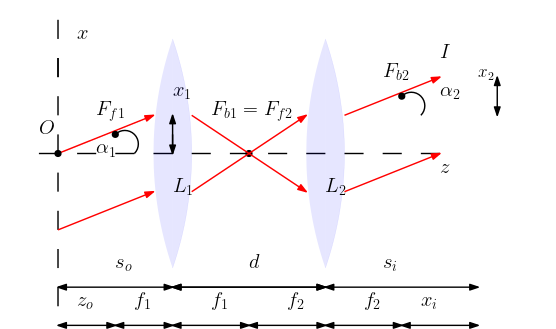
\includegraphics[height=2.0in]{figures/hw2/hw2_1.png}}
\caption{Parallel rays two lenses image formation variables spatial relationships}
\label{fig:2_1}
\end{figure}

\textbf{Exercise 1}\\
Parallel rays of elevation $x_1$ and propagation angle $\alpha_1$ are incident from the left on a two-lens system composed of two positive lenses $L1$ (focal length $f1>0$) and $L2$ (focal length $f2 >0)$ as shown in figure \ref{fig:2_1}.\\

\textbf{Q\&A} What is the distance between the lenses ($d$) as a function of the focal lengths in order for the ray bundle outgoing from the second lens to be parallel? In other words, to obtain collimated beam; image at infinite? \textbf{Hint:} Use Image formation principle.\\

%In a properly spaced two lens system an incoming collimated ray bundle  

Due to the thin lens approximation, the lens thickness of $L_1$ and $L_2$ is negligible and $\therefore$ for elevation on either side of the lens $x_L = x_R = x$ . The system is surrounded by air with index $n_{air} = 1$. The ray transfer matrix for $L_1$ is

\begin{equation}
\begin{bmatrix}
    \alpha_m \\
    x_2
\end{bmatrix}
=
\begin{bmatrix}
    1   &   0 \\
    d   &   1
\end{bmatrix}
\begin{bmatrix}
    1   & -\frac{1}{f_1} \\
    0   &   1
\end{bmatrix}
\begin{bmatrix}
     \alpha_{1} \\
    x_1
\end{bmatrix}
\end{equation}

and the ray transfer matrix for $L_2$ is

\begin{equation}
\begin{bmatrix}
    \alpha_2 \\
    x_2
\end{bmatrix}
=
\begin{bmatrix}
    1   & -\frac{1}{f_2} \\
    0   &   1
\end{bmatrix}
\begin{bmatrix}
    \alpha_{m}  \\
    x_2
\end{bmatrix}
\Rightarrow
\begin{bmatrix}
    1   & -\frac{1}{f_2} \\
    0   &   1
\end{bmatrix}^{-1}
\begin{bmatrix}
    \alpha_2 \\
    x_2
\end{bmatrix}
=
\begin{bmatrix}
    \alpha_{m}  \\
    x_2
\end{bmatrix}
\end{equation}

substitution of matrix \ref{} into matrix \ref{} results in

\begin{equation}
\begin{bmatrix}
    1   & -\frac{1}{f_2} \\
    0   &   1
\end{bmatrix}^{-1}
\begin{bmatrix}
    \alpha_2 \\
    x_2
\end{bmatrix}
=
\begin{bmatrix}
    1   &   0 \\
    d   &   1
\end{bmatrix}
\begin{bmatrix}
    1   & -\frac{1}{f_1} \\
    0   &   1
\end{bmatrix}
\begin{bmatrix}
     \alpha_{1} \\
    x_1
\end{bmatrix}
\end{equation}

solve for reciprocal matrix, and multiplying the matrices 

\begin{equation}
\begin{bmatrix}
    \alpha_2 + \frac{x_2}{f_2}\\
    x_2
\end{bmatrix}
=
\begin{bmatrix}
    1   & -\frac{1}{f_1} \\
    d   & 1 -\frac{d}{f_1}  
\end{bmatrix}
\begin{bmatrix}
    \alpha_{1} \\
    x_1
\end{bmatrix}
\end{equation}

multiplying the right hand side matrices again

\begin{equation}
\begin{bmatrix}
    \alpha_2 + \frac{x_2}{f_2}\\
    x_2
\end{bmatrix}
=
\begin{bmatrix}
    \alpha_1 - \frac{x_1}{f_1} \\
    d\alpha_1 + x_1 - \frac{x_1 d}{f_1}
\end{bmatrix}
\end{equation}

solve for the column vectors on left and right side\\

\begin{equation}
\sqrt{(\alpha_2 + \frac{x_2}{f_2})^2 + (x_2)^2} = \sqrt{(\alpha_1 - \frac{x_1}{f_1})^2 + (d\alpha_1 + x_1 - \frac{x_1 d}{f_1})^2}
\end{equation}

square both sides of equation and solve for d

\begin{equation}
\begin{aligned}
(\alpha_2 + \frac{x_2}{f_2})^2 + (x_2)^2 - (\alpha_1 - \frac{x_1}{f_1})^2 -x_1^2 & = d^2\alpha_1^2 + \frac{x_1^2 d^2}{f_1^2}\\ 
                                                                               & + d \alpha_1 x_1 - \frac{x_1^2 d}{f_1} - \frac{x_1^2 d^2 \alpha_1}{f_1}
\end{aligned}
\end{equation}

\begin{equation}
\begin{aligned}
(\alpha_2 + \frac{x_2}{f_2})^2 + (x_2)^2 - (\alpha_1 - \frac{x_1}{f_1})^2 -x_1^2 & = d^2(\alpha_1^2 + \frac{x_1^2}{f_1^2} - \frac{x_1^2\alpha_1}{f_1})\\ 
                                                                                 & + d(\alpha_1 x_1 - \frac{x_1^2}{f_1})
\end{aligned}
\end{equation}

square both sides of equation and solve for d and expand \\

Simplify with the knowledge that for the outgoing ray bundle from the second lens to be parallel $\alpha_1 = \alpha_2$ and $\therefore$ we can relabel $\alpha_1 = \alpha_2 =\alpha$.\\

\\ Trigonometrically we can state that $\tan(\alpha_m) = \frac{x_2}{d}$. For the outgoing ray bundle from the second lens to be parallel $\alpha_1 = \alpha_2$.\\

%\begin{equation}
%\begin{aligned}
%\alpha_2^2 + 2\frac{\alpha_2 x_2}{f_2} + \frac{x_2^2}{f_2^2} + x_2^2} = & \alpha_1^2 - 2\frac{\alpha_1 x_1}{f_1} + \frac{\alpha_1^2}{f_1^2} \\
% & + d^2\alpha_1^2 + x_1^2 + \frac{x_1^2 d^2}{f_1^2}\\ 
% & + d \alpha_1 x_1 - \frac{x_1^2 d}{f_1} - \frac{x_1^2 d^2 \alpha_1}{f_1}
%\end{aligned}
%\end{equation}


%solve for d

%\begin{equation}
%\begin{aligned%}
% \alpha_2^2 + 2\frac{\alpha_2 x_2}{f_2} + \frac{x_2^2}{f_2^2} + x_2^2}         & \\
% - \alpha_1^2 + 2\frac{\alpha_1 x_1}{f_1} - \frac{\alpha_1^2}{f_1^2} - x_1^2   & = d^2\alpha_1^2 + \frac{x_1^2 d^2}{f_1^2}\\ 
%                                                                               & + d \alpha_1 x_1 - \frac{x_1^2 d}{f_1} - \frac{x_1^2 d^2 \alpha_1}{f_1}
%\end{aligned}
%\end{equation}

%Simplify

%\begin{equation}
%\begin{aligned}
% \alpha_2^2 + 2\frac{\alpha_2 x_2}{f_2} + \frac{x_2^2}{f_2^2} + x_2^2}         & \\
% - \alpha_1^2 + 2\frac{\alpha_1 x_1}{f_1} - \frac{\alpha_1^2}{f_1^2} - x_1^2   & = d(d^2\alpha_1^2 + \frac{x_1^2 d^2}{f_1^2}\\ 
%                                                                               & + d \alpha_1 x_1 - \frac{x_1^2 d}{f_1} - \frac{x_1^2 d^2 \alpha_1}{f_1}
%\end{aligned}
%\end{equation}





\newpage

\textbf{Q\&A} What is the optical power of this composite optical system and effective focal length (also referred to as \textbf{element focal length})? What is the value of the optical power for $d=f1+f2$? \textbf{Hint:} RTM?\\

Optical power is equal to the reciprocal of the focal length of the device $P=\frac{1}{f}$. The element focal length for a two lens system is defined as $EFL = \frac{f_1 \times f_2}{f_1 + f_2 - d}$ $\therefore$ the optical power of a two lens system is defined as $P=\frac{f_1 + f_2 -d}{f_1 \times f_2}$ and $\therefore$ the optical power for $d=f_1 + f_2$ is shown to be $P=\frac{f_1 + f_2 - (f_1 + f_2)}{f_1 \times f_2} = 0$\\

\textbf{Q\&A} What are the propagation angle $\alpha_2$ and width $a_2$ (defined as $x_2$ in the figure \ref{fig:2_1} and matrices) of this outgoing ray bundle? \\

$\alpha_2$ and width(z in Joseph Crandall's coordinate system) $z_2$ are spatially indicated in figure \ref{fig:2_1}.\\

\textbf{Q\&A} What are the angular and lateral magnifications?\\

The angular magnification is defined as $M_A = \frac{-s_o}{s_1}$ and the lateral magnification (sometimes called linear or transverse) is defined as $M_T = \frac{-s_i}{s_o}$. $s_o$ and $s_i$ are indicated spatially in figure \ref{fig:2_1}\\

\textbf{Q\&A} How is the image (virtual, real), what about the object? (Please point them out)\\

Object $O$ and image $I$ are spatially indicated in figure \ref{fig:2_1}. The collimated rays are incident from $\infty$ at object $O$ and the collimated rays create a real image at $\infty$ at $I$. 


\newpage

\begin{figure}
\centering\fbox{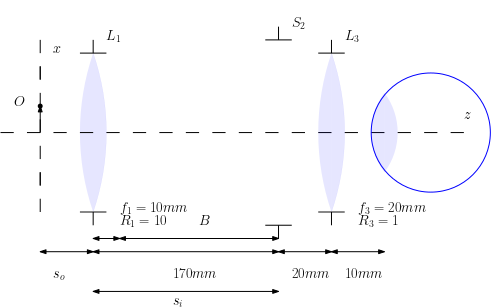
\includegraphics[height=2.0in]{figures/hw2/hw2_2.png}}
\caption{Spatial Relationships between lens, aperture, lens, eye}
\label{fig:2_2}
\end{figure}

\textbf{Exercise 2}\\
The optical instrument shown below consists of 2 lenses $L_1$, $L_3$ and an aperture stop $S_2$ and the observer's eye is located to the right of $L_3$. Symbols $\{f_1 , R_1\}$ , $\{f_3 , R_3\}$ represent the focal lengths and radii of $L_1$, $L_3$, respectively, and $R_2$ is the radius of $S_2$ \ref{fig:2_2}.\\

\textbf{Q\&A} Determine the object distance so that a human observer's unaccommodating eye (no strain for focusing) can focus the image on the observer's retina. \textbf{Hint:} this means outgoing parallel ray bundle from $L_3$, which means that lens $1 ...$\\

... must have incident object $O$ at $\infty$. \\

\textbf{Q\&A} What is the instrument use and what is the magnifying power? \textbf{Hint:} small object viewed by an eye

\end{document}